\section{Annotations}

All the source code of this section is available \href{https://github.com/LM-96/QA-Extensions/tree/main/it.unibo.qakactor/src/main/kotlin/annotations}{here}.

\subsection{The example case: \texttt{LedSonar} system}

Before talking about annotations, we show a small example that will be used to demonstrate some usages and to make some first approximated tests.

We will consider a simple case that is used in the course of \emph{Ingegneria Dei Sistemi Software}: a system with a \textcolor{MidnightBlue}{\textbf{led}} and a \textcolor{MidnightBlue}{\textbf{sonar}} connected to a single board computer like Raspberry.
\textbf{When the sonar detects a distance less than a threshold, the system must turn on the led. If the distance detected goes over this threshold, the led must be powered off}.

\begin{figure}[h]
	\centering
	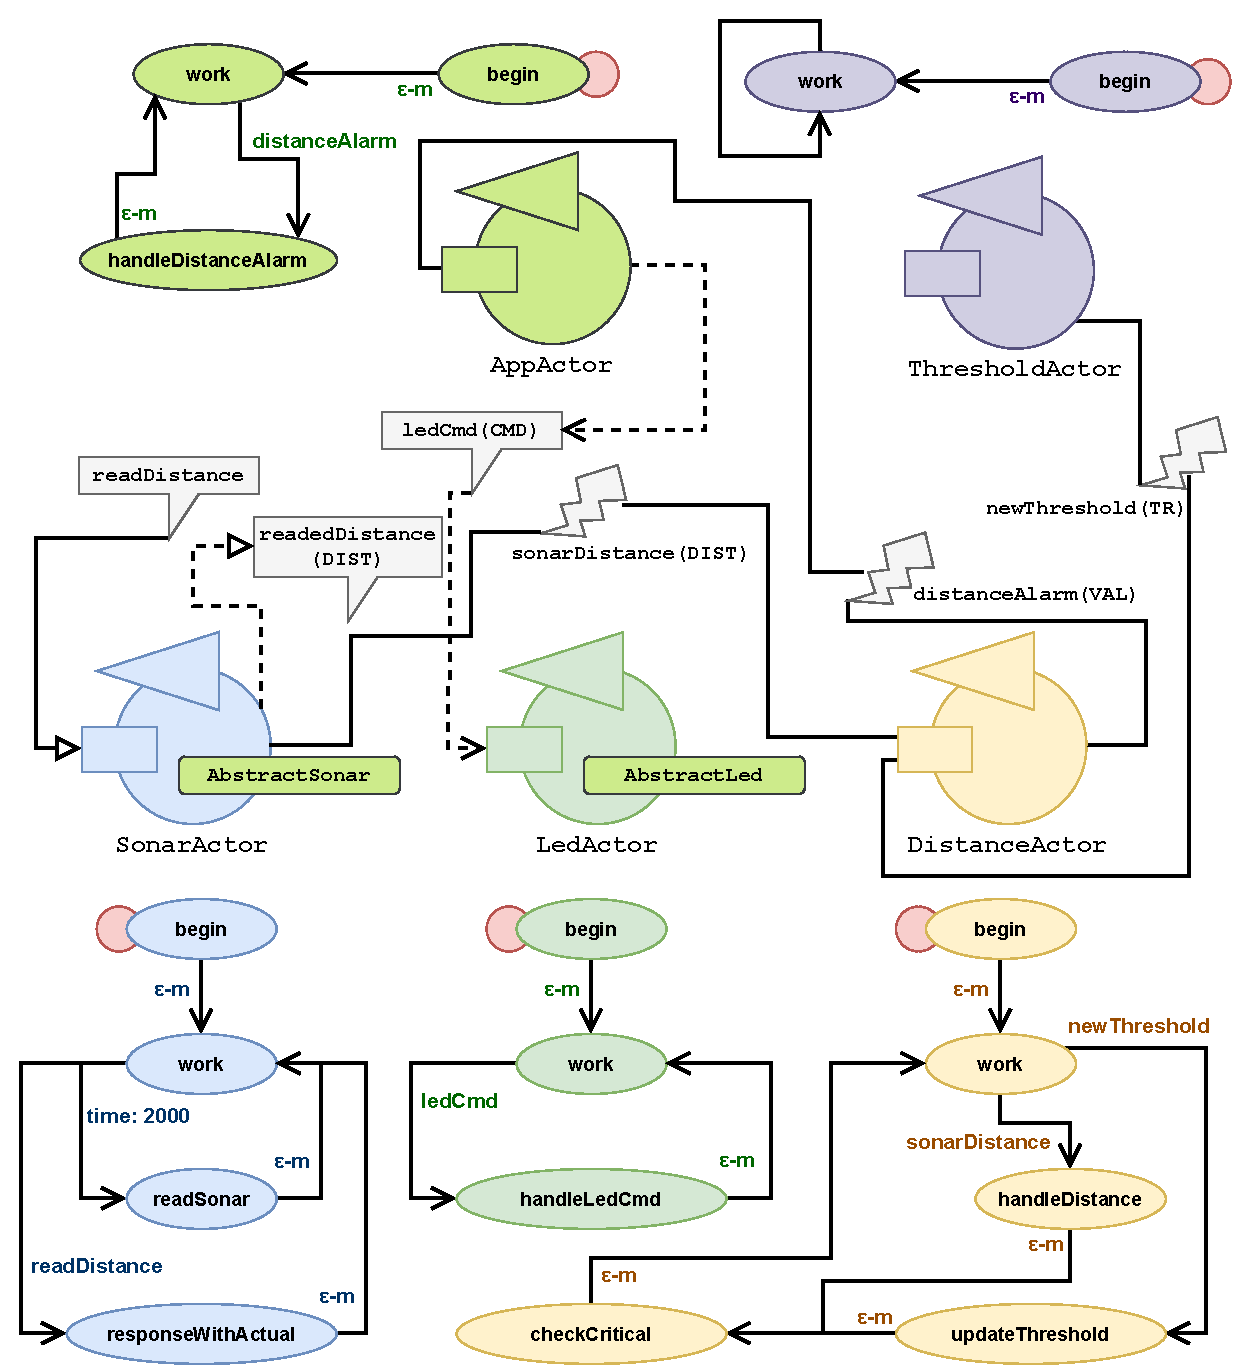
\includegraphics[width=\textwidth]{img/[EG]led_sonar_actor_diagram}
	\caption{Diagram of the \texttt{ledsonar} system}
	\label{fig::ledsonar_system}
\end{figure}

The figure \ref{fig::ledsonar_system} shows the diagram of the \texttt{ledsonar} system that will be used fot the examples. The legend of the used notation can be found \href{https://github.com/anatali/issLab2021/blob/main/it.unibo.issLabStart/userDocs/Legenda.pptx}{here}, 
but we will not go into the details of the logic.

In summary:
\begin{itemize}
	\item \underline{\texttt{SonarActor}}:\\
	This actor hold a sonar that it can use to read the value from it.
	The actor can receive request and answer to it but it also do polling emitting \texttt{sonarDistance} events with the current value of the distance read from the sonar.
	
	\item \underline{\texttt{LedActor}}:\\
	This actor hold a led that it can command.
	The actor can receive dispatch \texttt{ledCmd(CMD)} with two possible value: \texttt{ON} for power on the led and \texttt{OFF} for turn it off.
	
	\item \underline{\texttt{DistanceActor}}:\\
	This actor continuously monitors the distance emitted by the \texttt{SonarActor}: if the value is less then the threshold then emits a \texttt{distanceAlarm("CRITICAL")} event, otherwise if the the distance returns to a value greater than the threshold then it fires the event \texttt{distanceAlarm("NORMAL")}.
	
	\item \underline{\texttt{AppActor}}:\\
	This actor realizes the business logic of the example system. When a \texttt{distanceAlarm} event is detected then it command the led in the proper way following the logic we have already shown.
\end{itemize}

We also need a \textit{virtual environment} in order to test our example system. Then we have created a small \textit{web based} architecture that simulates a \textit{sonar} and a \textit{led} using \texttt{WebSocket}.
The source code of this small system made in \texttt{Kotlin} using \href{https://ktor.io/}{\texttt{Ktor}} can be found \href{https://github.com/LM-96/QA-Extensions/tree/main/it.unibo.ledsonarsystem}{here}.

\begin{figure}[h]
	\centering
	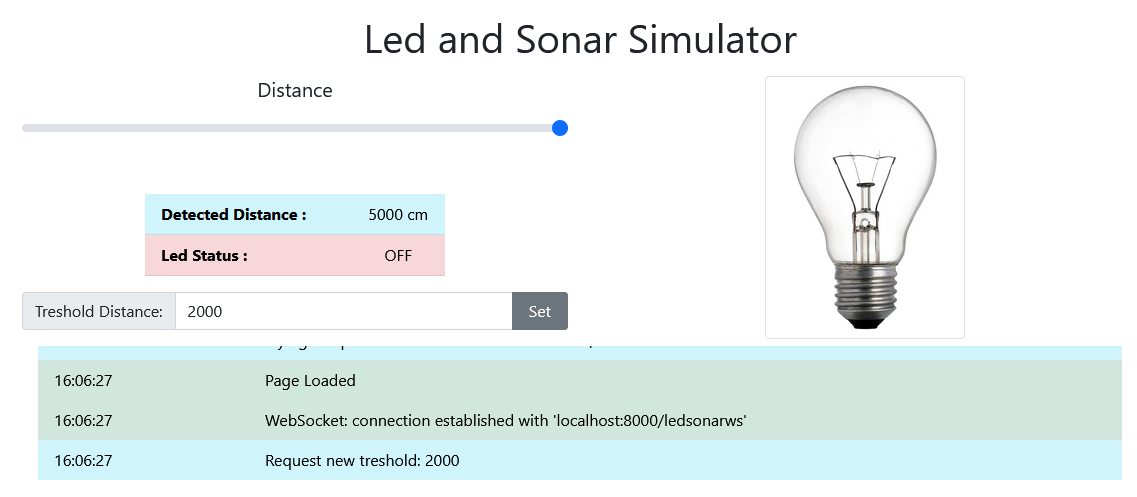
\includegraphics[width=\textwidth]{img/[EG]led_sonar_actor_gui}
	\caption{Web GUI of the \texttt{ledsonar} system}
	\label{fig::ledsonar_system_gui}
\end{figure}

When this system is started it possible to go at \href{http://localhost:8000/index.html}{localhost:8000/index.html} in order to get a small web based GUI that is shown in the figure \ref{fig::ledsonar_system_gui}.
The GUI use \texttt{WebSocket} in order to send new distances when the slider of the sonar is moved or to receive the command to power on/off the led. In particular, the GUI offers:

\begin{itemize}
	\item a \textcolor{ForestGreen}{\textbf{slider}} to modify the distance read from the sonar;
	
	\item a \textcolor{ForestGreen}{\textbf{box}} in which to type the new value of the threshold that can be sent over the WebSocket when the \texttt{Set} button is pressed;
	
	\item a \textcolor{ForestGreen}{\textbf{led image}} that shows when the led is powered on or off.
\end{itemize}

For this reason the actor system in the figure \ref{fig::ledsonar_system} contains an additional actor called \underline{\texttt{ThresholdActor}}: it listens the commands to update the threshold over the WebSocket and when a new value is received emits the proper event \texttt{newTreshold}.

In order to start this system it possible to call the \texttt{startLedSonarSystem()} function that is present in the file \href{https://github.com/LM-96/QA-Extensions/blob/main/it.unibo.ledsonarsystem/src/main/kotlin/it/unibo/ledsonarsystem/LedSonarSystem.kt}{LedSonarSystem.kt}.

If you want to use a real sonar or a real led you only have to extends properly the two \texttt{POJO} owned by the \texttt{SonarActor} and the \texttt{LedActor}.

\subsection{Descriptive annotations [ \href{https://github.com/LM-96/QA-Extensions/tree/main/it.unibo.ledsonardemo0}{\textcolor{Emerald}{\textbf{ledonarsystem0}}} ]}

The focus of our discussion is \textcolor{ForestGreen}{\textbf{to introduce a new mechanism do let the developer able to easily describe the system using annotations}}. The use of the annotation can be very useful:
\begin{itemize}
	\item they do not depend on an IDE and are included in Java so there are no compatibility problems;
	\item they can completely describe all the aspects of the actor system;
	\item the use of the annotations is very easy and intuitive.
\end{itemize}

So the first step is \textcolor{ForestGreen}{\textbf{to develop some annotations to eliminate the need for the \texttt{.pl} file}}. This annotations let the system able to find all the information about the contexts and the actors that are defined.

\begin{itemize}
	\item \href{https://github.com/LM-96/QA-Extensions/blob/main/it.unibo.qakactor/src/main/kotlin/annotations/QakContext.kt}{\textcolor{YellowOrange}{\underline{\texttt{QakContext}}}}:\\
	\textit{This annotation is applicable to a class and give to the system the information about a context (name, address, protocol and port).}
	\begin{lstlisting}[numbers=none,language=Kotlin]
		annotation class QakContext(
			val contextName : String,
			val contextAddress : String,
			val contextProtocol : String,
			val contextPort : Int,
		)
	\end{lstlisting}

	\item \href{https://github.com/LM-96/QA-Extensions/blob/main/it.unibo.qakactor/src/main/kotlin/annotations/QActor.kt}{\textcolor{YellowOrange}{\underline{\texttt{QActor}}}}:\\
	\textit{This annotation is applicable to a class that is an actor and then \textbf{it must extends \texttt{ActorBasic}}. It maintains all the information of the actor (name, context, ecc\dots)}
	\begin{lstlisting}[numbers=none,language=Kotlin]
		annotation class QActor(
			val contextName : String,
			val actorName : String = "",
			val discardMessage : Boolean = false,
			val confined : Boolean =  false,
			val ioBound : Boolean = false,
			val channelSize : Int = 50
		)
	\end{lstlisting}

	\item \href{https://github.com/LM-96/QA-Extensions/blob/main/it.unibo.qakactor/src/main/kotlin/annotations/QakContext.kt}{\textcolor{YellowOrange}{\underline{\texttt{Hostname}}}}:\\
	\textit{This annotation is applicable to a class and indicates the hostname of the system. This annotation is not strictly necessary but at the moment it's mandatory to identify the context that have to run locally.}
	\begin{lstlisting}[numbers=none,language=Kotlin]
		annotation class HostName(
			val hostname : String
		)
	\end{lstlisting}
\end{itemize}

Actually, there is no full support to the description of remote actors but in future development it is easy to add it.

Then, as explained the \textit{location} of the entities of the system can be describing using these annotations. The \href{https://github.com/LM-96/QA-Extensions/tree/main/it.unibo.ledsonardemo0}{\textcolor{Emerald}{\textbf{ledonarsystem0}}} example shows how it is possible to use them.
In this paper we just show the \href{https://github.com/LM-96/QA-Extensions/blob/main/it.unibo.ledsonardemo0/src/main/kotlin/it/unibo/ledsonardemo0/actors/SonarActor.kt}{SonarActor} end the \href{https://github.com/LM-96/QA-Extensions/blob/main/it.unibo.ledsonardemo0/src/main/kotlin/it/unibo/ledsonardemo0/actors/LedActor.kt}{LedActor}:

\begin{lstlisting}[caption=\texttt{SonarActor} (\texttt{ledsonarsystem0}),language=Kotlin]
@QActor("ctxLedSonarAbFsmDemo")
class SonarActor(name : String, scope : CoroutineScope) :
	ActorBasicFsm(name, scope, autoStart = false) {
	
	var distance = -1
	var prevDistance = distance
	val sonar = SYSTEM_SONAR
	
	override fun getBody(): ActorBasicFsm.() -> Unit {
		return {
			state("begin") {
				transition(edgeName = "t0", targetState = "work", cond = doswitch())
			}
			
			state("work") {
				action {
					stateTimer = TimerActor("timer_begin",
					scope, context!!, "local_tout_${name}_$stateName", 2000 )
				}
				transition(edgeName = "t1", targetState = "readSonar",
				cond = whenTimeout("local_tout_${name}_$stateName"))
				transition(edgeName = "t2", targetState = "answareWithActual",
				cond = whenRequest("readDistance"))
			}
			
			state("readSonar") {
				action {
					prevDistance = distance
					distance = sonar.read()
					if(prevDistance != distance) {
						emit("sonarDistance", "sonarDistance($distance)")
					}
				}
				transition(edgeName = "t3", targetState = "work", cond = doswitch())
			}
			
			state("answareWithActual") {
				action {
					replyToCaller("readDistance", "readDistance($distance)")
				}
				transition(edgeName = "t4", targetState = "work", cond = doswitch())
			}
		}
	}
	
	override fun getInitialState(): String {
		return "begin"
	}
	
}
\end{lstlisting}

\begin{lstlisting}[caption=\texttt{LedActor (\texttt{ledsonarsystem0})},language=Kotlin]
@QActor("ctxLedSonarAbFsmDemo")
class LedActor(name : String, scope : CoroutineScope) :
	ActorBasicFsm(name, scope, autoStart = false) {

	val led = SYSTEM_LED

	override fun getBody(): ActorBasicFsm.() -> Unit {
		return {
			
			state("begin") {
				action {}
				transition(edgeName = "t0", targetState = "work", cond = doswitch())
			}
			
			state("work") {
				action {}
				transition(edgeName = "t1", targetState = "handleLedCmd",
					cond = whenDispatch("ledCmd"))
			}
			
			state("handleLedCmd") {
				action {
					try {
						if(checkMsgContent(
							Term.createTerm("ledCmd(CMD)"),
							Term.createTerm("ledCmd(CMD)"),
							currentMsg.msgContent()))
						when(val ledCmdArg = payloadArg(0)) {
							"OFF", "off" -> {
								if(led.isPoweredOn()) {led.powerOff()}
							}
							"ON", "on" -> {
								if(led.isPoweredOff()) {led.powerOn()}
							}
						}
					} catch (e : Exception) {/* ... */}
				}
				transition(edgeName = "t2", targetState = "work", cond = doswitch())
			}
		}
	}

	override fun getInitialState(): String {
		return "begin"
	}
}
\end{lstlisting}

With the others class that we have not reported here, the description of the actors of the system is completed. But the system can not be started yet because there are nothing able to make it run reading the annotations. It is needed a component that \textbf{scans all the classes and load the annotated one}.
Indeed, we have developed a new component called \href{https://github.com/LM-96/QA-Extensions/blob/main/it.unibo.qakactor/src/main/kotlin/annotations/AnnotationLoader.kt}{\textcolor{ForestGreen}{\texttt{AnnotationLoader}}} with the method 
\begin{center}
	\begin{tabular}{c}
		\begin{lstlisting}[frame=none,numbers=none,language=Kotlin]
			fun loadSystemByAnnotations(params : ReadableParameterMap
						= immutableParameterMap()) : SystemBuilder
		\end{lstlisting}
	\end{tabular}
\end{center}

This method \textbf{scan all classes of the application and search for annotated} loading them depending on the annotation. We have also added a component called \href{https://github.com/LM-96/QA-Extensions/blob/main/it.unibo.qakactor/src/main/kotlin/QakLauncher.kt}{\textcolor{ForestGreen}{\texttt{QakLauncher.kt}}} with proper methods that launch the system calling the \texttt{AnnotationLoader}. So the \texttt{Kotlin} script that launches the system is:

\begin{lstlisting}[caption=\texttt{App.kt} (\texttt{ledsonarsystem0}), language=Kotlin]
@QakContext("ctxLedSonarAbFsmDemo", "localhost", "TCP",9000)
@HostName("localhost")
class ContextConfiguration

fun main(args: Array<String>) {
	startLedSonarSystem()
	
	runBlocking {/*this:CoroutineScope*/
		launchQak(this)
	}
}
\end{lstlisting}

Notice that this mechanism is added to the infrastructure as an extension and without invalidating the old \texttt{.pl} definition. 

\subsection{New classes for injection}

We remember that \href{https://github.com/anatali/issLab2021/blob/main/it.unibo.qakactor/src/main/kotlin/ActorBasic.kt}{ActorBasic} and \href{https://github.com/anatali/issLab2021/blob/main/it.unibo.qakactor/src/main/kotlin/ActorBasicFsm.kt}{ActorBasicFsm} classes are \textit{abstract} so it is not possible to directly create instances of this classes because of the \textit{abstract} definition.
For this reason we have created the two classes shown in the previous section and that are used from the builders: \texttt{ActorBasicWrapper} and \texttt{ActorBasicFsmWrapper} that takes the transient actor definitions and wrap them into \texttt{ActorBasic} or \texttt{ActorBasicFsm} instances.

Now it is clear that a level of strong separation has been introduced between the \textcolor{ForestGreen}{\textbf{\textit{definition}}} of the actor system and the \textcolor{ForestGreen}{\textbf{\textit{runnable implementation}}} of it.

In addition to this, the new \texttt{@QActor} annotation allow the developer to specify the actor's name directly into the proper annotation field. So, if the developer is forced to directly extends the \texttt{ActorBasic} class, he must always specify a constructor with the two parameter needed by the superclass as done in the previous listings.

We want not only to avoid this but also to introduce \textbf{a new stronger level of separation} between the runnable part of the actor (represented by the \texttt{ActorBasic} inherited type) and the description (represented by the override of the proper methods).

\begin{figure}[h]
	\centering
	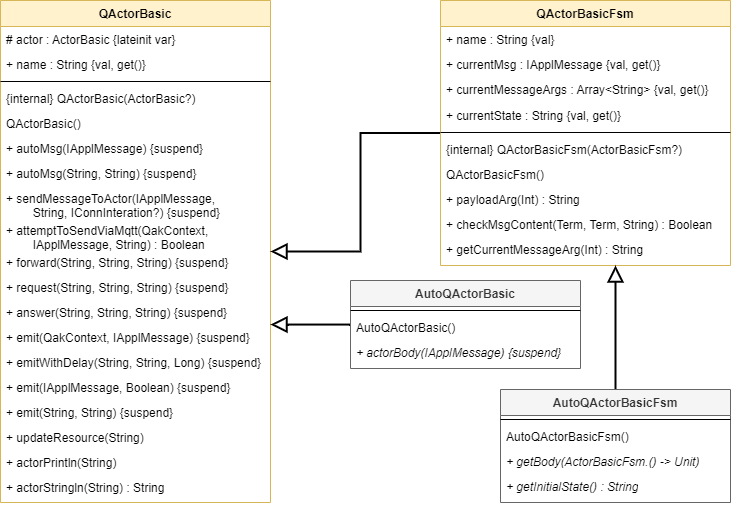
\includegraphics[width=\textwidth]{img/[UML]QActorBasic_QActorBasicFsm_Auto}
	\caption{\texttt{Q} and \texttt{AutoQ} classes}
	\label{fig::q_autoq_classes}
\end{figure}

Then, first, we have created new classes in order to realize the separation: \href{https://github.com/LM-96/QA-Extensions/blob/main/it.unibo.qakactor/src/main/kotlin/QActorBasic.kt}{\texttt{QActorBasic}} and \href{https://github.com/LM-96/QA-Extensions/blob/main/it.unibo.qakactor/src/main/kotlin/QActorBasicFsm.kt}{\texttt{QActorBasicFsm}}. These two classes are illustrated in the figure \ref{fig::q_autoq_classes} can be used in order to define the behaviour of the actors (\textit{basic} or finite state machine) by extending them and adding other mechanisms such as some proper annotations that will be shown.

However, the application designer can decide to insert some operations inside the behaviour that requires to be invoked on the \textit{runnable instance} of the actor he is developing. For this reason, the \texttt{QActorBasic} must anyway maintain the \textit{runnable part} that is the \texttt{ActorBasic} instance (and the correspondent \texttt{ActorBasicFsm} for the \texttt{QActorBasicFsm}) that unfortunately should be available only after the instantiation of the \texttt{Q} classes.

As shown in figure \ref{fig::q_autoq_classes}, the main operations that require the executable instance are related with sending messages and events or performing \texttt{CoAP} updates or \texttt{Mqtt} interactions.

The \texttt{QActorBasic} and \texttt{QActorBasicFsm} classes are very useful in order to define new methods for describing the behaviour of the actors, but they do not provide a full and complete mechanism for this.
What the developer needs to put inside these classes? And above all, how it is possible to initialize the \texttt{ActorBasic} variable inside?

We will answer to the first question in the next subsection. Indeed, for the second, we can say that the most easy and useful way to put the \texttt{ActorBasic} instance is by using reflection. So, the application designer writes the code to create an actor using \texttt{QActorBasic} and then the component able to load the class instantiates the related \texttt{ActorBasic} instance and inject it to the \texttt{Q} class.

\subsection{\texttt{AutoQ} classes  [ \href{https://github.com/LM-96/QA-Extensions/tree/main/it.unibo.ledsonardemo1}{\textcolor{Emerald}{\textbf{ledonarsystem1}}} ]}

In the figure \ref{fig::q_autoq_classes} are present two new classes that we have not clarified: \href{https://github.com/LM-96/QA-Extensions/blob/main/it.unibo.qakactor/src/main/kotlin/AutoQActorBasic.kt}{\texttt{AutoQActorBasic}} and \href{https://github.com/LM-96/QA-Extensions/blob/main/it.unibo.qakactor/src/main/kotlin/AutoQActorBasicFsm.kt}{\texttt{AutoQActorBasicFsm}}. They are very simple because their only work is to let the application designer to use the \textit{legacy} actor definition with the \textit{descriptive annotation} without forcing him to use the classical constructor of the \texttt{ActorBasic} or \texttt{ActorBasicFsm} classes.

So, \textcolor{ForestGreen}{\textbf{it is possible to use the \texttt{@QActor} annotation with a class that extends \texttt{AutoQActorBasic}}} without specifying any parameter in the superclass constructor (and in this sense it is \textit{auto}).

